\section{Verstärker-Schaltungen}


\subsection{Verstärker für Hochton-Bereich}
\subsubsection{Allgemeines}\label{subsec:4.5.1}
Die gefilterten Hochton-Frequenzen müssen vor dem Abstrahlen verstärkt werden.
Hierfür wird die TDA2030-Verstärker-Grundschaltung(siehe Kapitel \ref{subsec:3.2.2}) verwendet.
\\ \\
%TDA2030 Grundschaltung Verweis
Hier ohne Leistungstransistoren, da Hochton-Lautsprecher nicht eine so hohe Leistung, ohne Gefahr von Zerstörung, umsetzen können.
Die Spulen des Lautsprechers könnten bei zu hoher Leistung durchbrennen, d.h. der Isolierschutzlack der Spulenwindungen wird zu heiß, die Windungen werden kurzgeschlossen.
Das verstärkte Audiosignal weist dadurch am Ausgang der Schaltung eine höhere Spannung und einen höheren Strom auf.
\\ \\
Es soll nach diesem Schritt möglich sein den Hochton-Lautsprecher in einer der zwei Satellitenboxen mit ausreichend Signal zu versorgen, um einen Schalldruck von zumindest Zimmerlautstärke zu erhalten. 
% Sollen wir hier genau das selbe schreiben wie beim TTVerstärker?

\newpage
\subsubsection{Schaltung}\label{subsec:4.5.2}
Aus der TDA2030-Grundschaltung (siehe Kapitel \ref{subsec:3.2.2}) folgend ist auch hier ein Spannungsteiler vorgesehen um den Arbeitspunkt (Siehe Kapitel \ref{subsec:3.5.1}) einzustellen.
%TDA2030 Grundschaltung Verweis + Arbeitspunkt Verweis
Die Schaltung wurde aus dem Datenblatt übernommen, nur vereinzelte Werte wurden angepasst. 
% Veränderte Werte nennen?

\begin{figure} [H]
	\centering	
	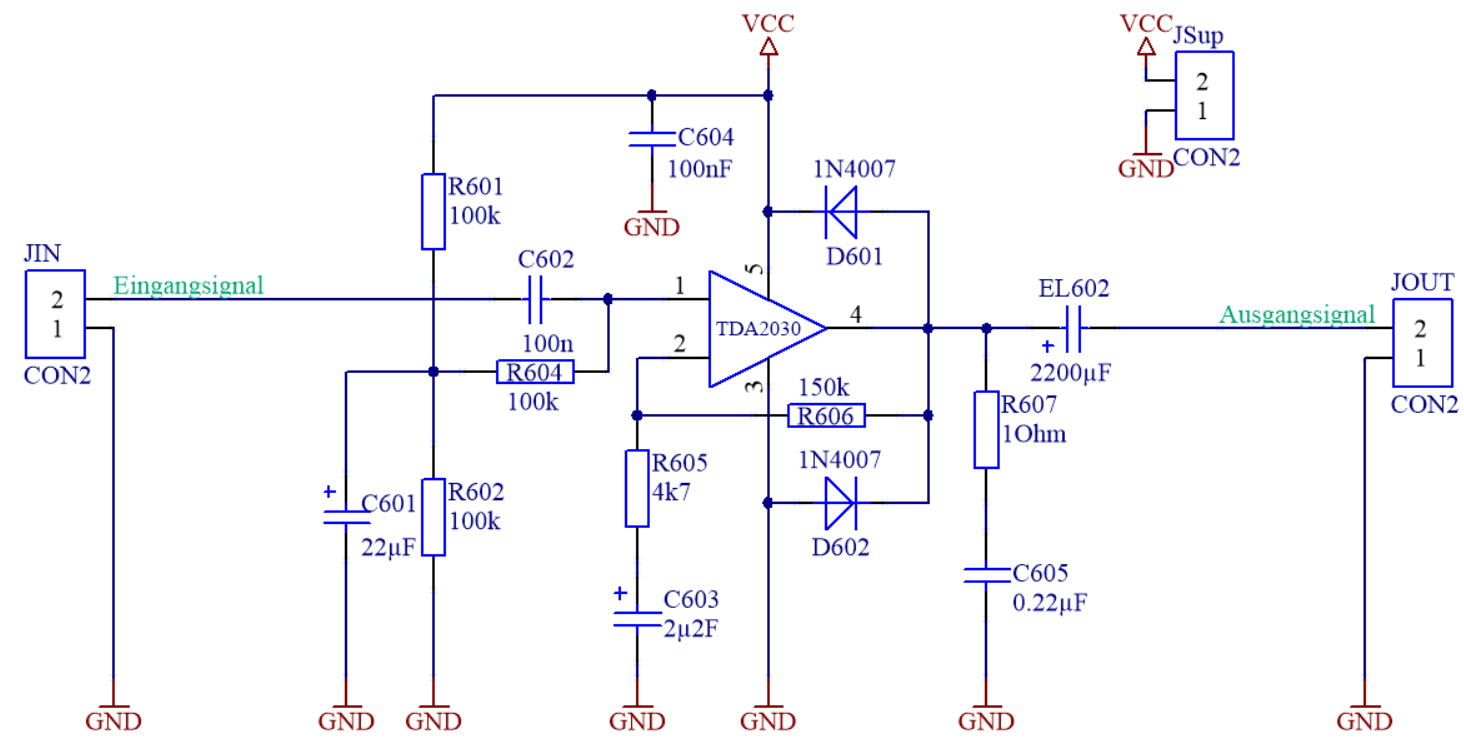
\includegraphics[width=1\textwidth]{img/Print6/HTVerstaerker-Schem.PNG}
	\caption{Verstärker für Hochton-Bereich - Schaltung}
	\label {fig:4.5.2.1}
\end{figure}

\newpage
\subsubsection{PCB}\label{subsec:4.5.3}
Das Layout wird wieder nach den Grunddesignregeln(siehe Kapitel \ref{subsec:3.1.2}) erstellt.\\
%TD Grunddesignregel Verweis
Eine große Fläche über dem TDA2030 wird vorgesehen um einen Testkühlkörper mit dem Print mechanisch verbinden zu können.
Es dient zur Verringerung der Hebelwirkung.
%Mit Fortschreiten der Arbeit wurde die Fläche gekürtzt um mit dem neuen Kühlkörper eben abzuschließen.

\begin{figure} [H]
	\centering	
	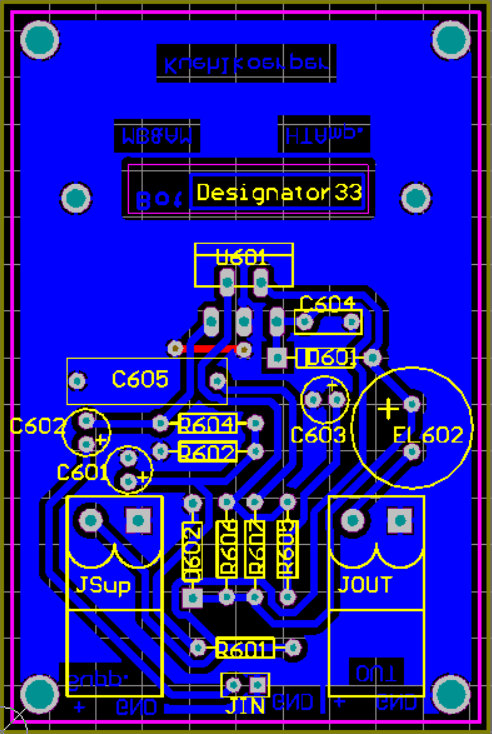
\includegraphics[width=0.7\textwidth]{img/Print6/HTVerstaerker-PCB.PNG}
	\caption{Verstärker für Hochton-Bereich - PCB}
	\label {fig:4.5.3.1}
\end{figure}


\newpage
\subsection{Verstärker für Tiefton-Bereich}
\subsubsection{Allgemeines}\label{subsec:4.4.1}
Nach dem Filtern des Signals soll dieses vor dem Abstrahlen am Lautsprecher verstärkt werden.
Es wurde eine analoge Verstärker-Schaltung verwendet, da diese einfacher und mit weniger Problemen realisiert werden konnte.
\\ \\
Mithilfe bereits bekannter, bewährter Schaltungen konnte ein Layout für diese Schaltung entwickelt werden.
Ein wichtiger Baustein in dieser Schaltung ist der Verstärkerbaustein \enquote{TDA2030} (Siehe Kapitel \ref{sec:3.2}).
%TDA2030 Verweis
Des weiteren werden zwei Leistungstransistoren verbaut die höhere Ströme schalten können, falls der maximale Schaltstrom des TDA2030 erreicht wird (Siehe Kapitel \ref{subsec:3.2.3}).
\\ \\
%TDA2030 MaxRatings
Das Eingangssignal soll verstärkt werden um am Ausgang der Schaltung höhere Spannung und höheren Ströme aufzuweisen.
Es soll nach diesem Schritt möglich sein den Tiefton-Lautsprecher in einer der zwei Satellitenboxen mit ausreichend Signal zu versorgen, um einen Schalldruck von zumindest Zimmerlautstärke zu erhalten. 
%TD TDA2030 Verweis
%TD TDA2030-Maximum-Ratings Verweis

\newpage
\subsubsection{Schaltung}\label{subsec:4.4.2}
In der linken, oberen Ecke der Schaltung (\ref{fig:4.4.2.1}) ist der Spannungsteiler für einstellen des Arbeitspunktes (Siehe Kapitel \ref{subsec:3.5.1}) ersichtlich.
Mit Hilfe des ELKO's \enquote{EL504} wird verschleppte Gleichspannung am Eingang der Schaltung heraus gesiebt.
Dafür ist auch der ELKO \enquote{EL502}, dieser siebt die Gleichspannung am Ausgang der Schaltung heraus, bevor das Signal die Platine verlässt. \\
Über die Widerstände \enquote{R506} und \enquote{R505} wird die Verstärkung der Schaltung eingestellt.
In diesem Fall ist die Verstärkung $\frac{R505+R506}{R505}$ = 31 .
Das bedeutet, dass das Eingangssignal am Ausgang 31mal so groß sein soll, natürlich unter Beachtung der Grenzen der OPV-Verstärkerschaltung (\ref{sec:3.5}).
%TD Arbeitspunkt Verweis
%TD OPV-Verstärkerschaltung Verweis
%TD Layout TT-Verst

\begin{figure} [H]
	\centering	
	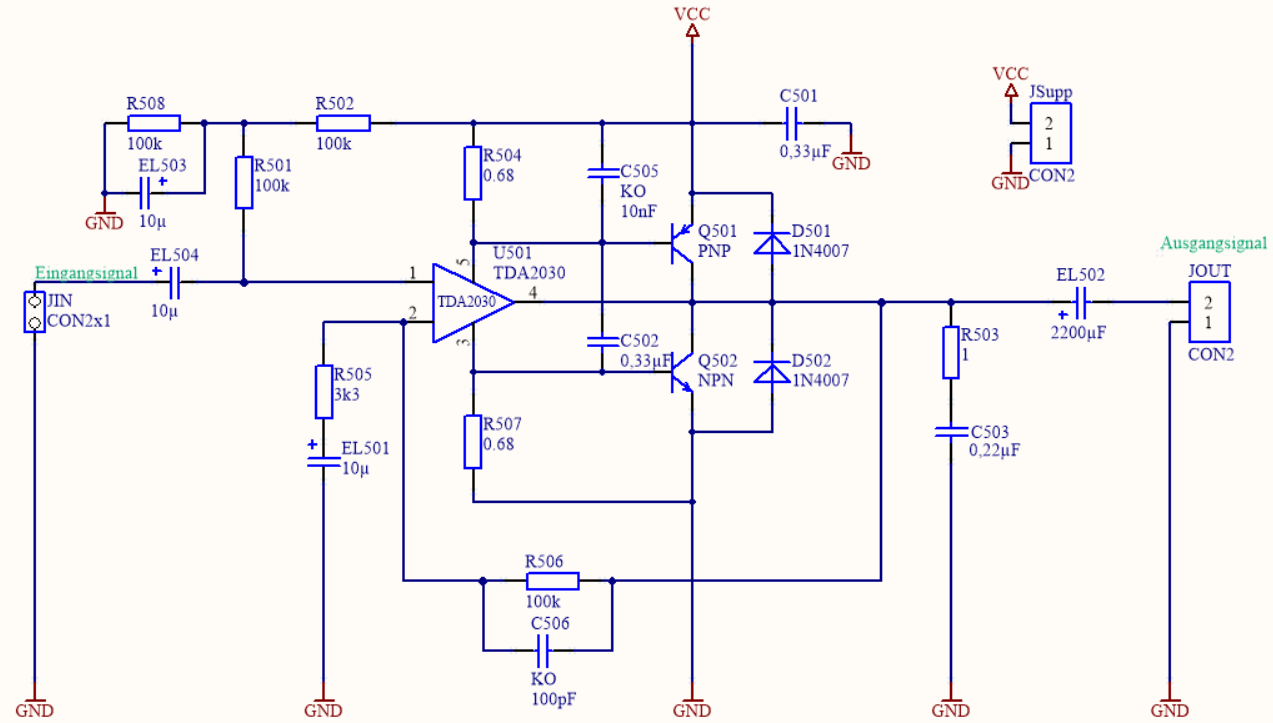
\includegraphics[width=1\textwidth]{img/Print5/5_TTVerstaerker-Schem.PNG}
	\caption{Verstärker für Tiefton-Bereich - Schaltung}
	\label {fig:4.4.2.1}
\end{figure}

\newpage
\subsubsection{PCB}\label{subsec:4.4.3}
Die drei zu kühlenden Bauteile \enquote{Q502, U501, Q501} (\ref{fig:4.4.3.1}) sind auf selber Höhe montiert um sie auf einen Kühlkörper montieren können.
\emph{Zu beachten dabei ist deren Potential an der Kühlfläche!}
Das Potential ist das Selbe wie an dem mittleren Anschluss-Pin des jeweiligen Bauteils.
Daher:
\begin{itemize}
	\item TDA2030: \enquote{-Vcc} = Masse bei asymmetrische Versorgung
	\item PNP(Q501): \enquote{Kollektor} = Ausgangssignal TDA2030
	\item NPN(Q502): \enquote{Kollektor} = Ausgangssignal TDA2030
\end{itemize}

Aus diesem Grund müssen zumindest die zwei Transistoren isoliert am Kühlkörper angebracht werden.\\
Die Ein- und Ausgänge sind auf einer Seite montiert. 
Einheitlich mit der Hochton-Verstärkerplatine(\ref{sec:4.5}) ist von links nach rechts zuerst Versorgungsstecker, dann Eingangssignal und am Ende der Ausgangsstecker angebracht.
Ebenso ist Masse jeweils rechts angeordnet um die Einheitlichkeit noch weiter zu erhöhen.\\
Auf der Platine ist über den zu kühlenden Elementen ist eine große frei Fläche mit Bohrungen um eine bessere mechanische Verbindung mit dem Kühlkörper zu erhalten.
Die vier kleineren Bohrungen waren für einen Testkühlkörper vorgesehen. 
Dieser Kühlkörper wurde bald durch einen größeren ersetzt, um mehrere Platinen montieren zu können.
%Die finale Ausführung ist jedoch nur auf die mechanische Verbindung der Bauteile mit dem Kühlkörper angewiesen.

\begin{figure} [H]
	\centering	
	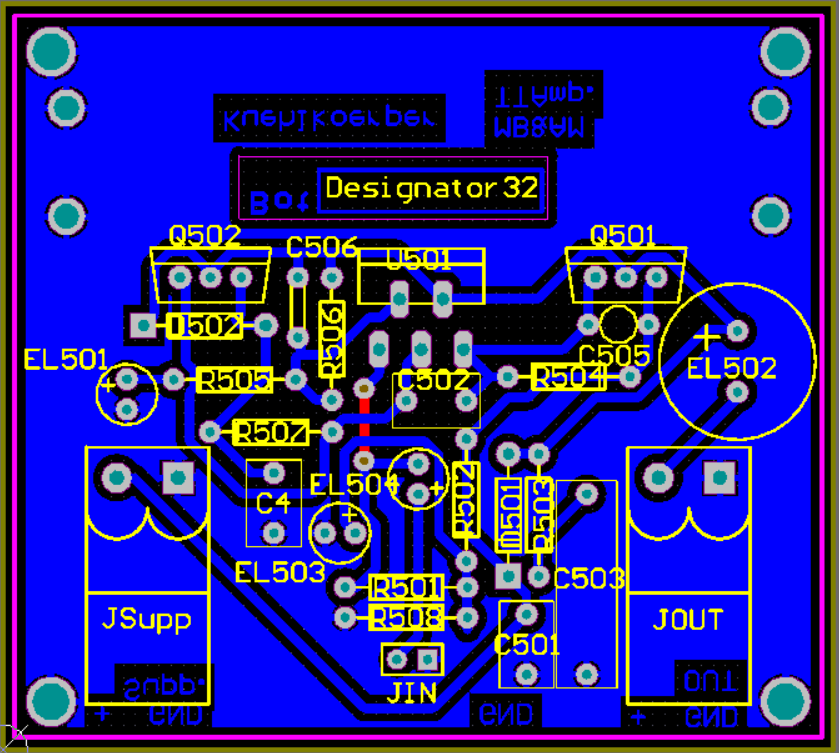
\includegraphics[width=0.6\textwidth]{img/Print5/5_TTVerstaerker-PCB.PNG}
	\caption{Verstärker für Tiefton-Bereich - PCB}
	\label {fig:4.4.3.1}
\end{figure}


\newpage
\subsection{Subwoofer-Verstärker}
Die Schaltung für den Verstärker wurde aus dem Datenblatt übernommen. %Verbindung mit H-Brücken "Grundlage"
Das bewährte Layout wurde aus einer HiFi-Zeitschrift übernommen (Artikel von: Herbert Sax).
%TD Subwoofer-Verst-Grundschaltung Verweis (alteGrundlagen)S